On the following pages of this appendix, there are plots of the results in Chapter~\ref{sec:efficiency_tests}.


\begin{figure}[ht]
    \centering
    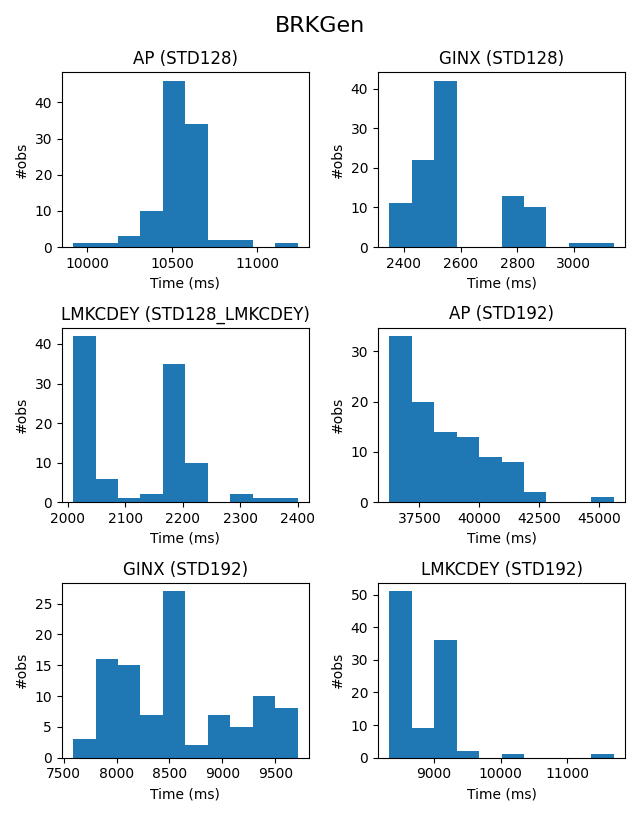
\includegraphics[width=\textwidth]{data/figures/BRKGen_distributions_1.png}
    \caption{Time distributions for different \texttt{OpenFHE} algorithms and different parameter sets when doing Test S1 (key generation) 100 times (see Chapter \ref{sec:efficiency_tests}).}
    \label{fig:distr_brkgen1}
\end{figure}

\begin{figure}[ht]
    \centering
    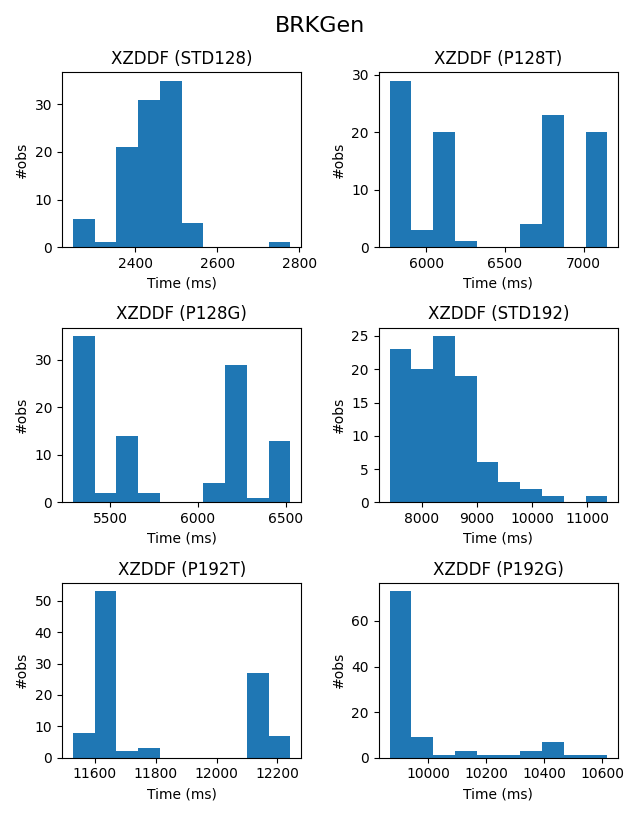
\includegraphics[width=\textwidth]{data/figures/BRKGen_distributions_2.png}
    \caption{Time distributions for XZDDF with different parameter sets when doing Test S1 (key generation) 100 times (see Chapter \ref{sec:efficiency_tests}).}
    \label{fig:distr_brkgen2}
\end{figure}


\begin{figure}[ht]
    \centering
    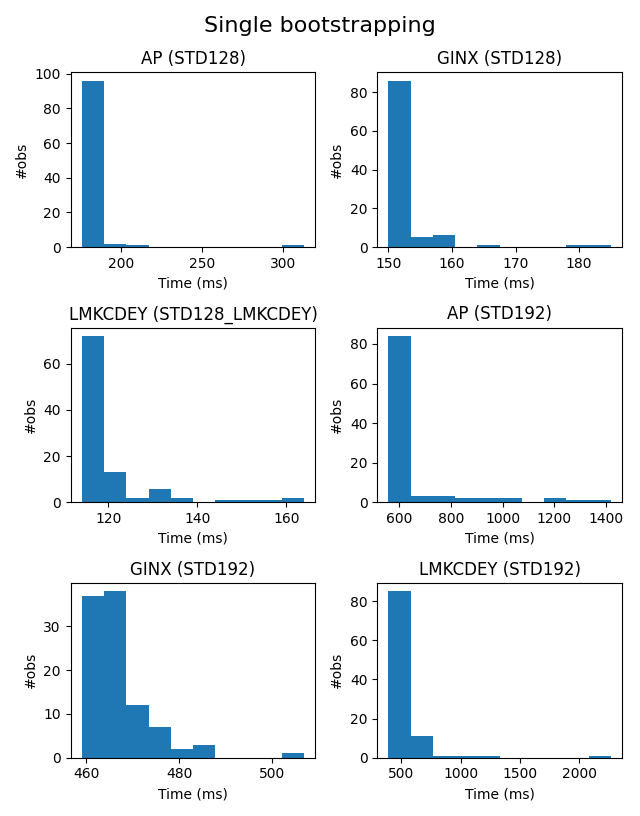
\includegraphics[width=\textwidth]{data/figures/Single_bootstrapping_distributions_1.png}
    \caption{Time distributions for different \texttt{OpenFHE} algorithms and different parameter sets when doing Test S2 (single bootstrapping) 100 times (see Chapter \ref{sec:efficiency_tests}).}
    \label{fig:distr_single_bootstrap1}
\end{figure}

\begin{figure}[ht]
    \centering
    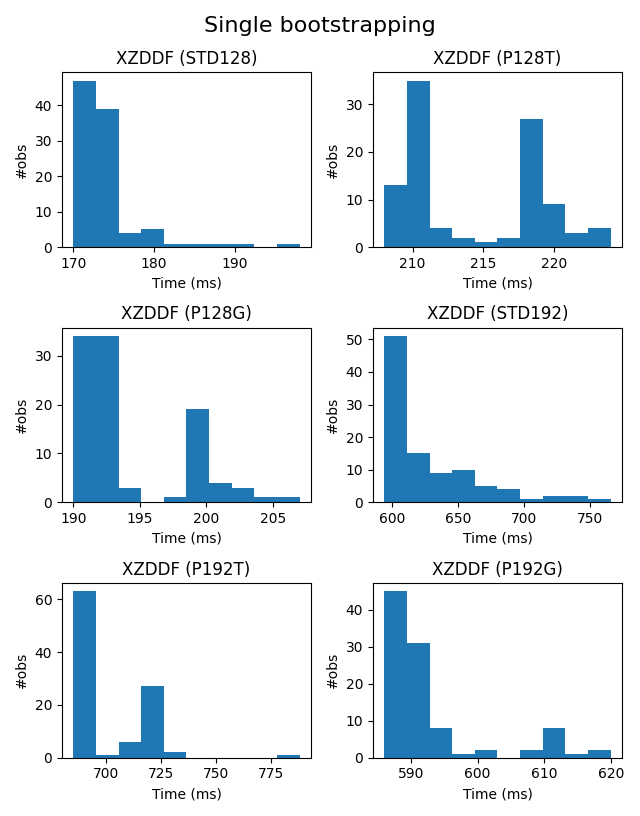
\includegraphics[width=\textwidth]{data/figures/Single_bootstrapping_distributions_2.png}
    \caption{Time distributions for XZDDF with different parameter sets when doing Test S2 (single bootstrapping) 100 times (see Chapter \ref{sec:efficiency_tests}).}
    \label{fig:distr_single_bootstrap2}
\end{figure}


\begin{figure}[ht]
    \centering
    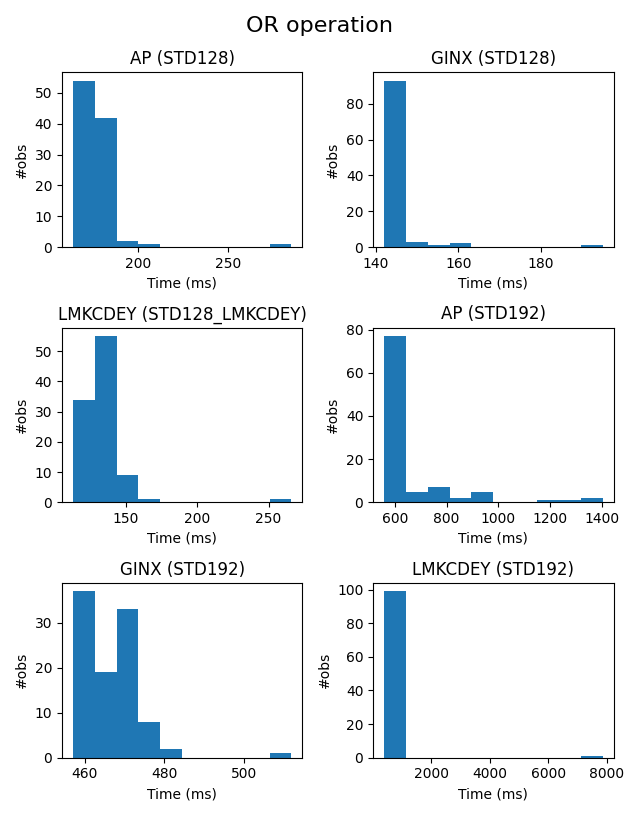
\includegraphics[width=\textwidth]{data/figures/OR_operation_distributions_1.png}
    \caption{Time distributions for different \texttt{OpenFHE} algorithms and different parameter sets when doing Test S3 (OR operation) 100 times (see Chapter \ref{sec:efficiency_tests}).}
    \label{fig:distr_or1}
\end{figure}

\begin{figure}[ht]
    \centering
    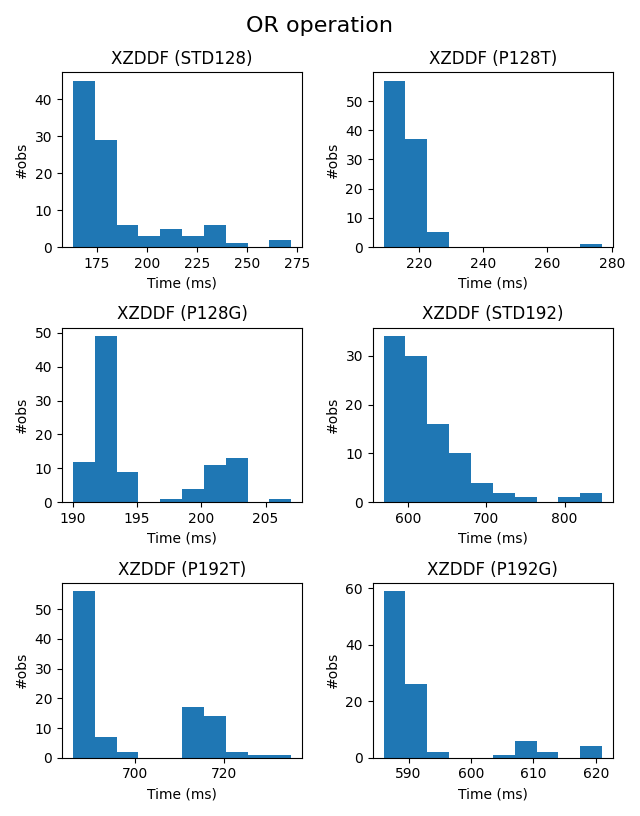
\includegraphics[width=\textwidth]{data/figures/OR_operation_distributions_2.png}
    \caption{Time distributions for XZDDF with different parameter sets when doing Test S3 (OR operation) 100 times (see Chapter \ref{sec:efficiency_tests}).}
    \label{fig:distr_or2}
\end{figure}


\begin{figure}[ht]
    \centering
    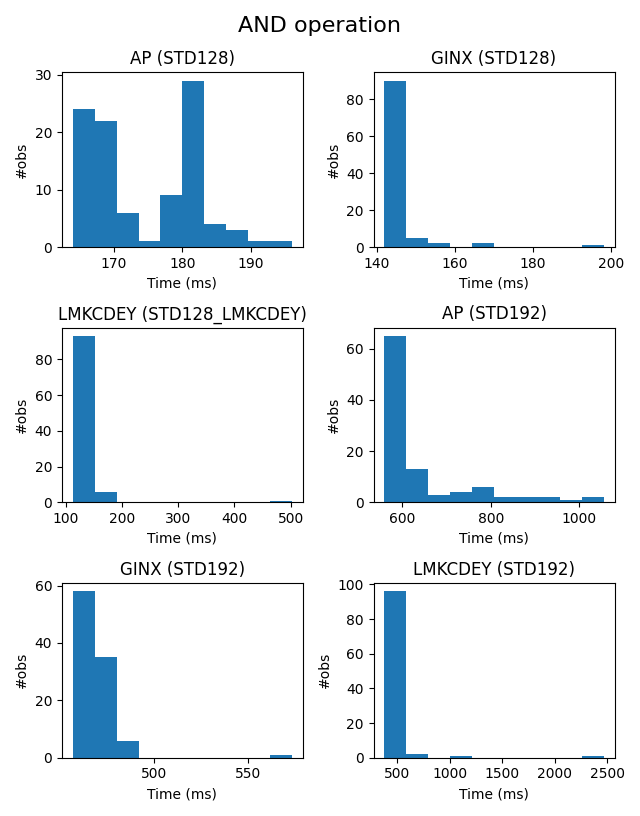
\includegraphics[width=\textwidth]{data/figures/AND_operation_distributions_1.png}
    \caption{Time distributions for different \texttt{OpenFHE} algorithms and different parameter sets when doing Test S4 (AND operation) 100 times (see Chapter \ref{sec:efficiency_tests}).}
    \label{fig:distr_and1}
\end{figure}

\begin{figure}[ht]
    \centering
    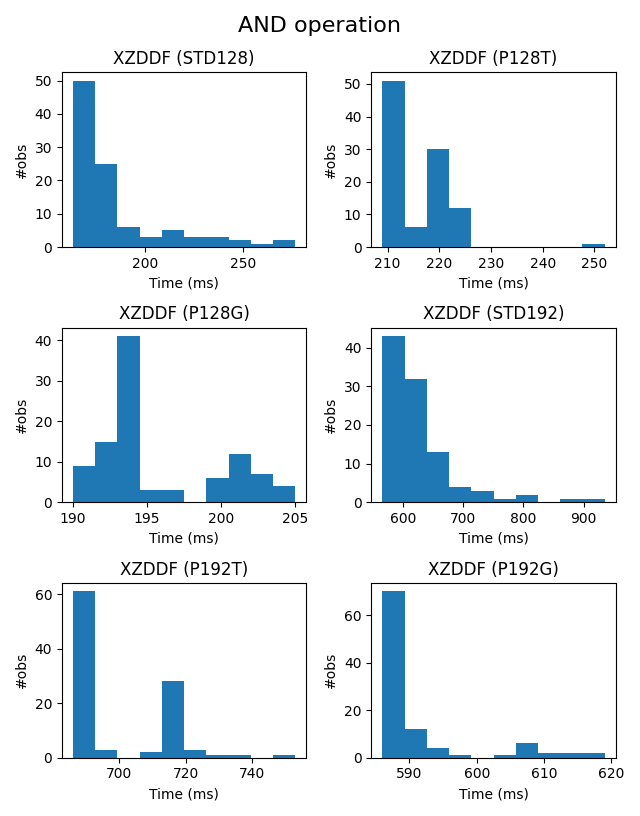
\includegraphics[width=\textwidth]{data/figures/AND_operation_distributions_2.png}
    \caption{Time distributions for XZDDF with different parameter sets when doing Test S4 (AND operation) 100 times (see Chapter \ref{sec:efficiency_tests}).}
    \label{fig:distr_and2}
\end{figure}


\begin{figure}[ht]
    \centering
    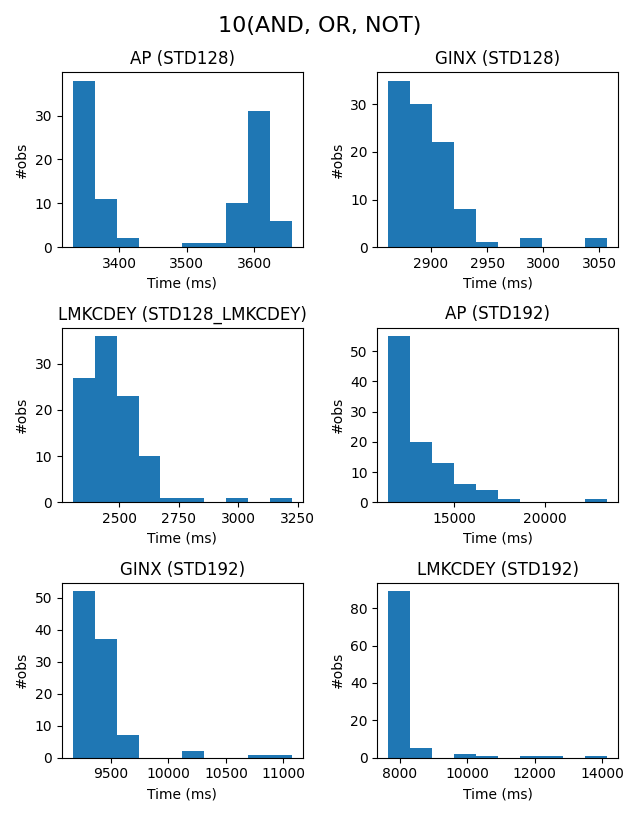
\includegraphics[width=\textwidth]{data/figures/10AND_OR_NOT_distributions_1.png}
    \caption{Time distributions for different \texttt{OpenFHE} algorithms and different parameter sets when doing Test B2 (10 AND, OR, and NOT operations) 100 times (see Chapter \ref{sec:efficiency_tests}).}
    \label{fig:distr_10andornot1}
\end{figure}

\begin{figure}[ht]
    \centering
    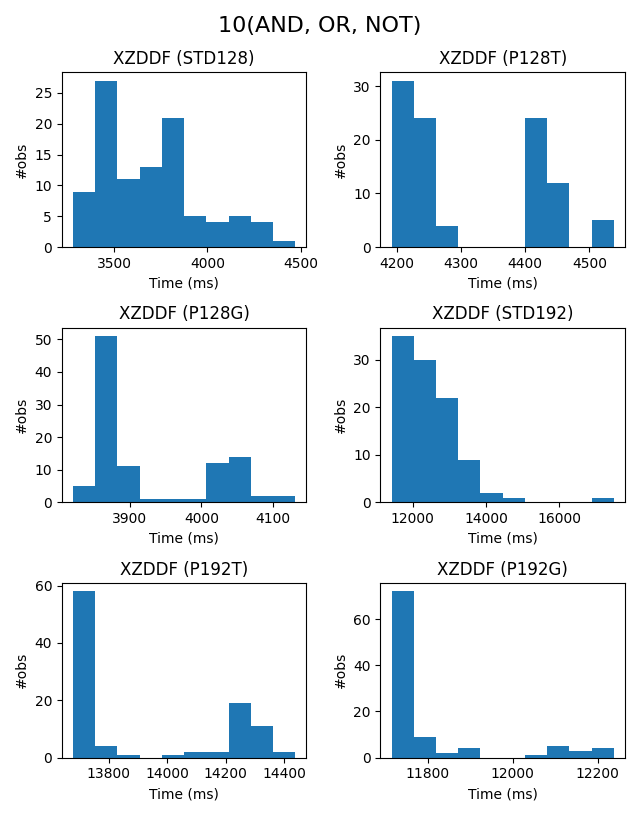
\includegraphics[width=\textwidth]{data/figures/10AND_OR_NOT_distributions_2.png}
    \caption{Time distributions for XZDDF with different parameter sets when doing Test B2 (10 AND, OR, and NOT operations) 100 times (see Chapter \ref{sec:efficiency_tests}).}
    \label{fig:distr_10andornot2}
\end{figure}


\begin{figure}[ht]
    \centering
    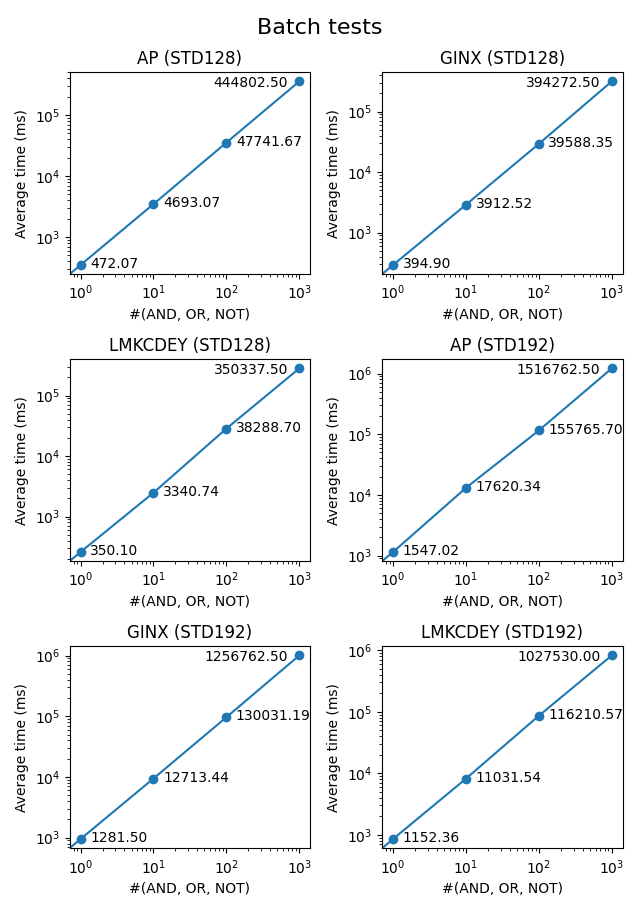
\includegraphics[width=\textwidth]{data/figures/batch_1.png}
    \caption{Log-log plots of the average execution times for different \texttt{OpenFHE} algorithms and different parameter sets when doing the batch tests B1--B4 in Chapter \ref{sec:efficiency_tests}, consisting of $x$ AND, OR, and NOT operations.}
    \label{fig:batch1}
\end{figure}

\begin{figure}[ht]
    \centering
    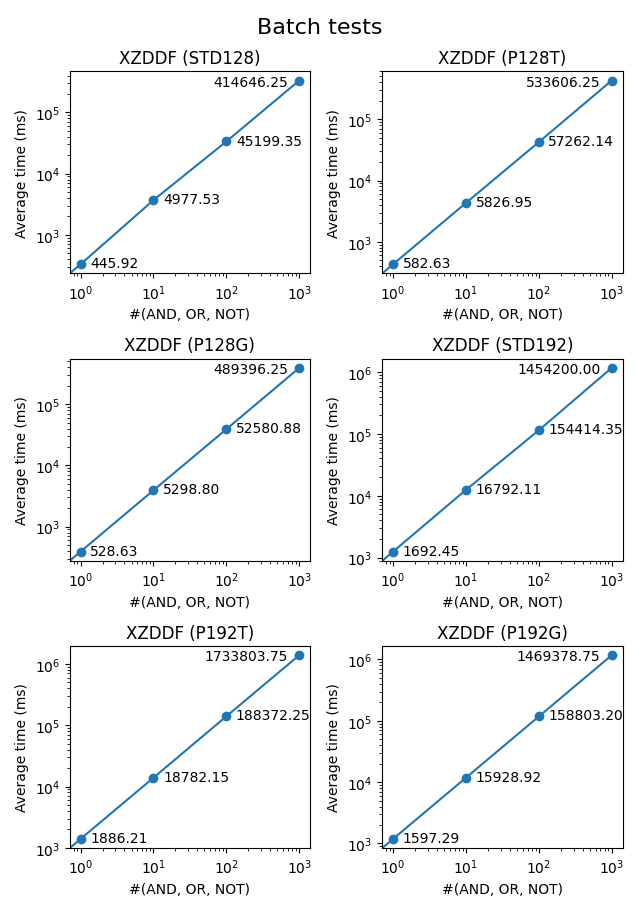
\includegraphics[width=\textwidth]{data/figures/batch_2.png}
    \caption{Log-log plots of the average execution times for XZDDF with different parameter sets when doing the batch tests B1--B4 in Chapter \ref{sec:efficiency_tests}, consisting of $x$ AND, OR, and NOT operations.}
    \label{fig:batch2}
\end{figure}



\iffalse

\begin{figure}[ht]
    \centering
    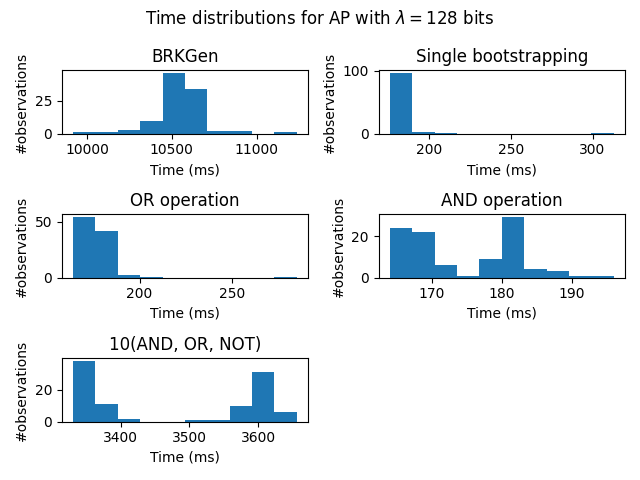
\includegraphics[width=\textwidth]{data/figures/AP_STD128_distributions.png}
    \caption{Time distributions when doing Test S1--S4 and Test B2 in Chapter \ref{sec:efficiency_tests} for 128 bits secure AP 100 times.}
    \label{fig:distr_ap128}
\end{figure}

\begin{figure}[ht]
    \centering
    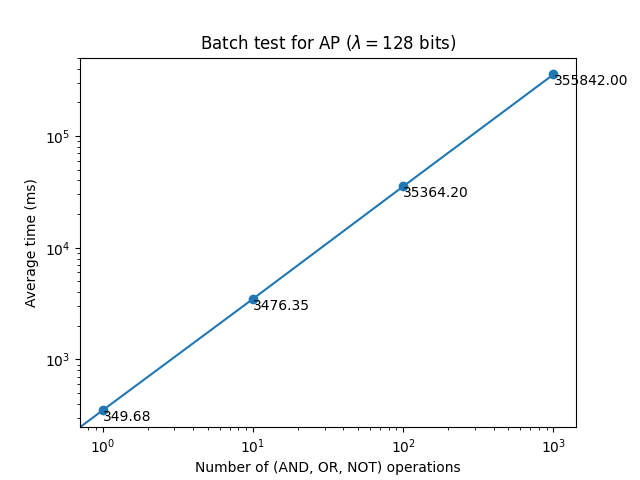
\includegraphics[width=0.8\linewidth]{data/figures/AP_STD128_batch.png}
    \caption{Log-log plot of the average execution times in the batch tests B1--B4 in Chapter \ref{sec:efficiency_tests} consisting of $x$ AND, OR, and NOT operations, for 128 bits secure AP.}
    \label{fig:batch_ap128}
\end{figure}

\begin{figure}[ht]
    \centering
    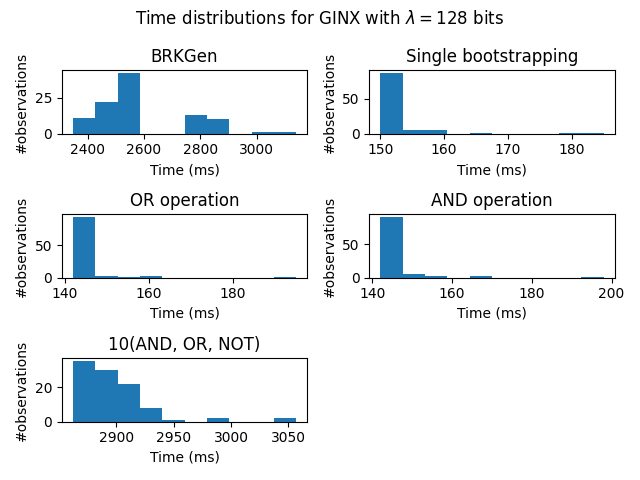
\includegraphics[width=\textwidth]{data/figures/GINX_STD128_distributions.png}
    \caption{Time distributions when doing Test S1--S4 and Test B2 in Chapter \ref{sec:efficiency_tests} for 128 bits secure GINX 100 times.}
    \label{fig:distr_ginx128}
\end{figure}

\begin{figure}[ht]
    \centering
    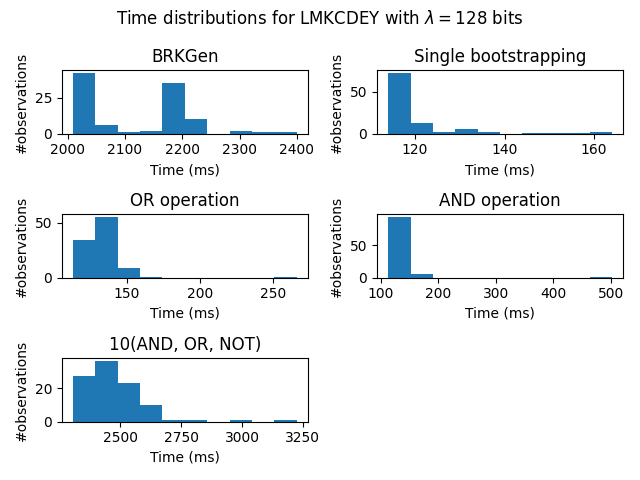
\includegraphics[width=\textwidth]{data/figures/LMKCDEY_STD128LMKCDEY_distributions.png}
    \caption{Time distributions when doing Test S1--S4 and Test B2 in Chapter \ref{sec:efficiency_tests} for 128 bits secure LMKCDEY 100 times.}
    \label{fig:distr_lmkcdey128}
\end{figure}

\begin{figure}[ht]
    \centering
    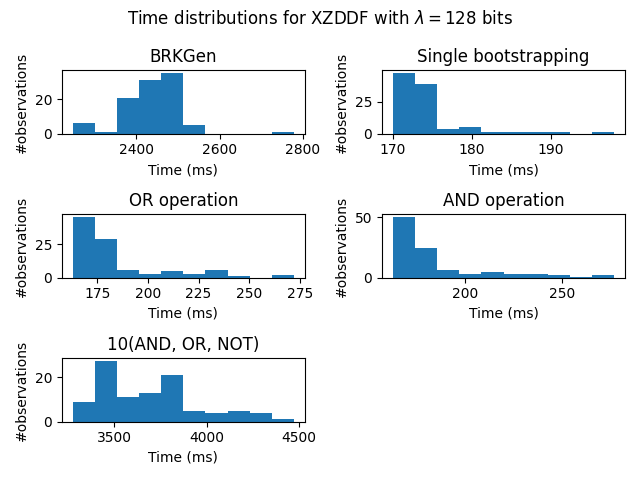
\includegraphics[width=\textwidth]{data/figures/XZDDF_STD128_distributions.png}
    \caption{Time distributions when doing Test S1--S4 and Test B2 in Chapter \ref{sec:efficiency_tests} for 128 bits secure XZDDF 100 times.}
    \label{fig:distr_xzddf128}
\end{figure}

\begin{figure}[ht]
    \centering
    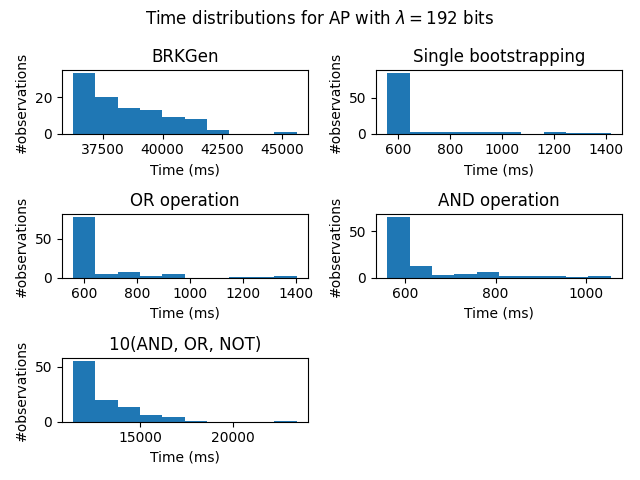
\includegraphics[width=\textwidth]{data/figures/AP_STD192_distributions.png}
    \caption{Time distributions when doing Test S1--S4 and Test B2 in Chapter \ref{sec:efficiency_tests} for 192 bits secure AP 100 times.}
    \label{fig:distr_ap192}
\end{figure}

\begin{figure}[ht]
    \centering
    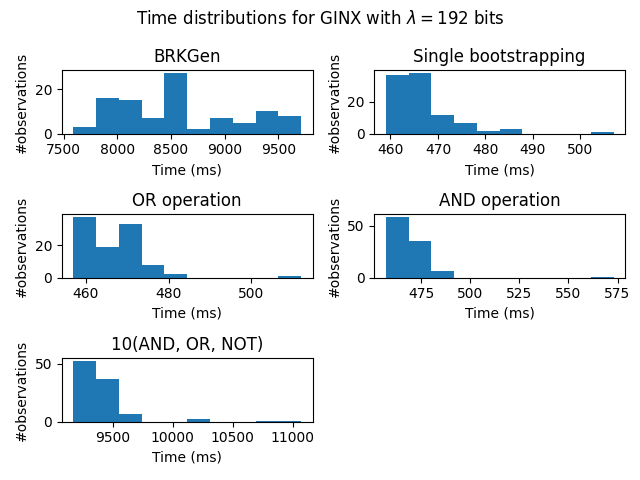
\includegraphics[width=\textwidth]{data/figures/GINX_STD192_distributions.png}
    \caption{Time distributions when doing Test S1--S4 and Test B2 in Chapter \ref{sec:efficiency_tests} for 192 bits secure GINX 100 times.}
    \label{fig:distr_ginx192}
\end{figure}

\begin{figure}[ht]
    \centering
    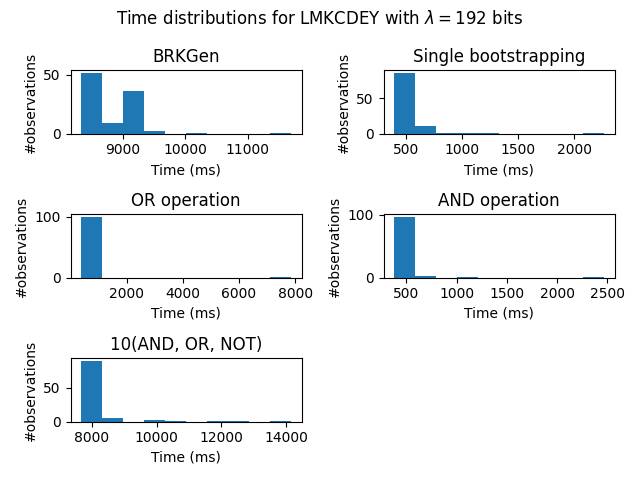
\includegraphics[width=\textwidth]{data/figures/LMKCDEY_STD192_distributions.png}
    \caption{Time distributions when doing Test S1--S4 and Test B2 in Chapter \ref{sec:efficiency_tests} for 192 bits secure LMKCDEY 100 times.}
    \label{fig:distr_lmkcdey192}
\end{figure}

\begin{figure}[ht]
    \centering
    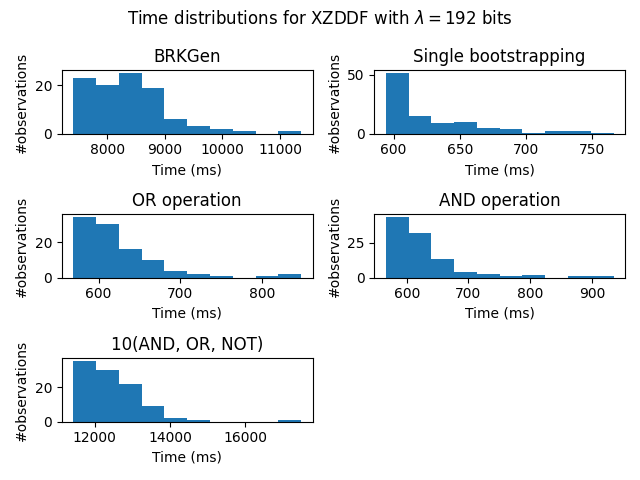
\includegraphics[width=\textwidth]{data/figures/XZDDF_STD192_distributions.png}
    \caption{Time distributions when doing Test S1--S4 and Test B2 in Chapter \ref{sec:efficiency_tests} for 192 bits secure XZDDF 100 times.}
    \label{fig:distr_xzddf192}
\end{figure}

% \begin{figure}
% \centering
% \begin{subfigure}{0.48\textwidth}
%     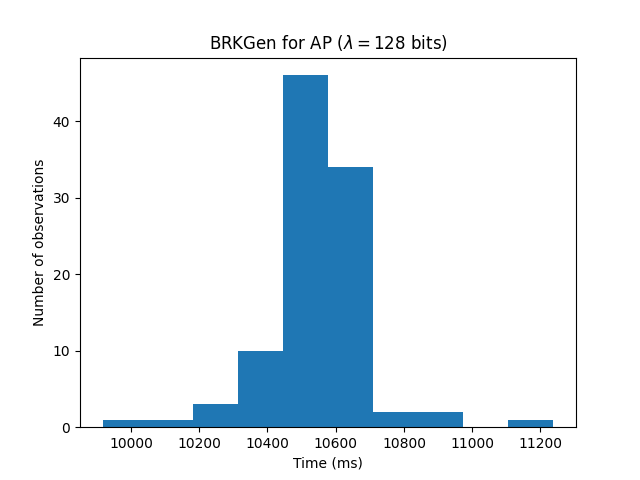
\includegraphics[width=\textwidth]{data/figures/AP_STD128_BRKGen.png}
%     \caption{Time distribution when doing Test S1 (key generation) in Chapter \ref{sec:efficiency_tests} for 128 bits secure AP 100 times.}
%     \label{fig:first}
% \end{subfigure}
% \hfill
% \begin{subfigure}{0.48\textwidth}
%     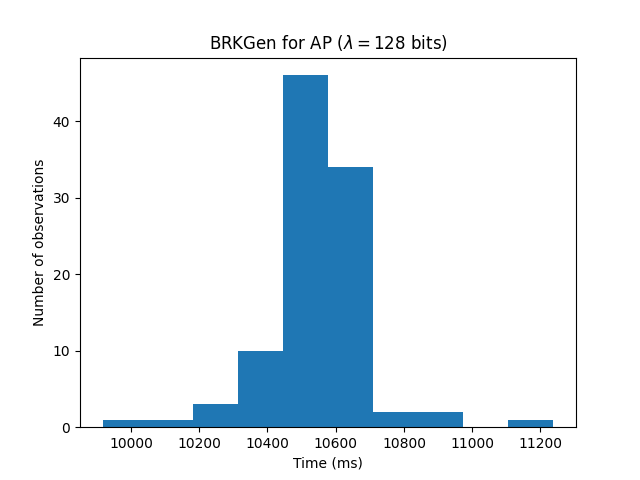
\includegraphics[width=\textwidth]{data/figures/AP_STD128_BRKGen.png}
%     \caption{Time distribution when doing Test S1 (key generation) in Chapter \ref{sec:efficiency_tests} for 128 bits secure AP 100 times.}
%     \label{fig:second}
% \end{subfigure}
% \hfill
% \begin{subfigure}{0.48\textwidth}
%     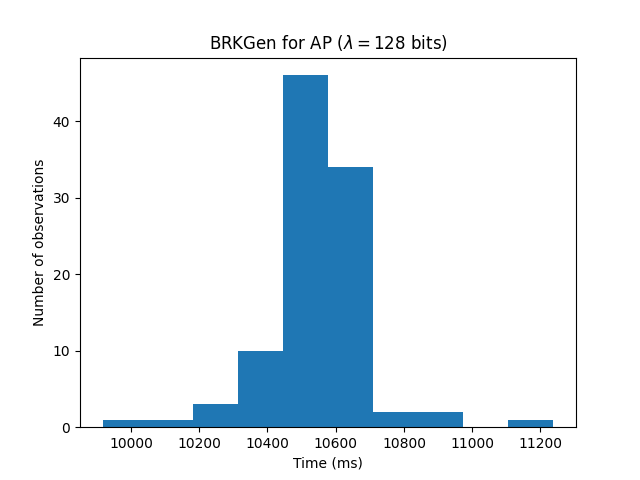
\includegraphics[width=\textwidth]{data/figures/AP_STD128_BRKGen.png}
%     \caption{Time distribution when doing Test S1 (key generation) in Chapter \ref{sec:efficiency_tests} for 128 bits secure AP 100 times.}
%     \label{fig:third}
% \end{subfigure}
        
% \caption{Creating subfigures in \LaTeX.}
% \label{fig:figures}
% \end{figure}



%%%%%%%% AP 128 %%%%%%%%
\begin{figure}[ht]
    \centering
    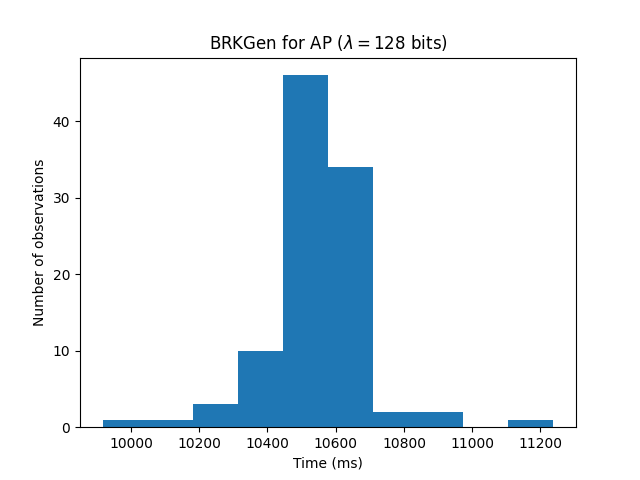
\includegraphics[width=0.8\linewidth]{data/figures/AP_STD128_BRKGen.png}
    \caption{Time distribution when doing Test S1 (key generation) in Chapter \ref{sec:efficiency_tests} for 128 bits secure AP 100 times.}
    \label{fig:distr_ap128_keygen}
\end{figure}

\begin{figure}[ht]
    \centering
    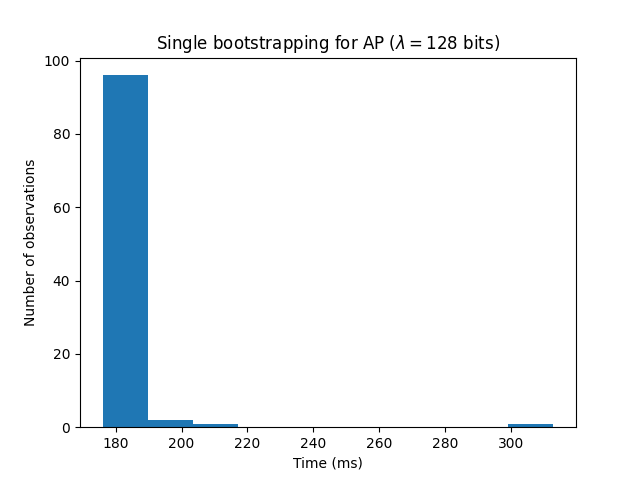
\includegraphics[width=0.8\linewidth]{data/figures/AP_STD128_Single_bootstrapping.png}
    \caption{Time distribution when doing Test S2 (single bootstrapping operation) in Chapter \ref{sec:efficiency_tests} for 128 bits secure AP 100 times.}
    \label{fig:distr_ap128_bs}
\end{figure}

\begin{figure}[ht]
    \centering
    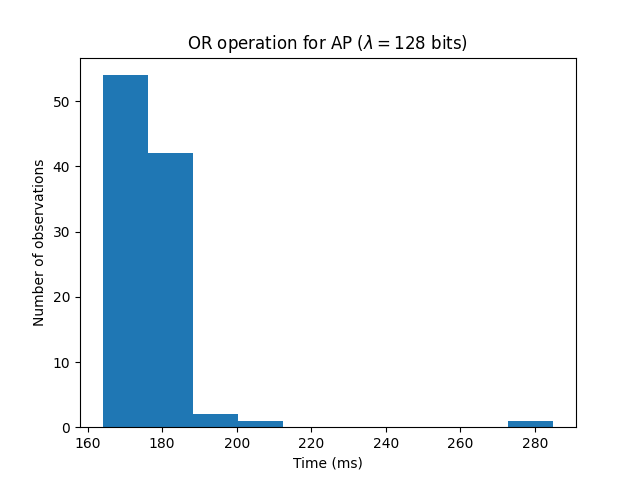
\includegraphics[width=0.8\linewidth]{data/figures/AP_STD128_OR_operation.png}
    \caption{Time distribution when doing Test S3 (OR operation) in Chapter \ref{sec:efficiency_tests} for 128 bits secure AP 100 times.}
    \label{fig:distr_ap128_or}
\end{figure}

\begin{figure}[ht]
    \centering
    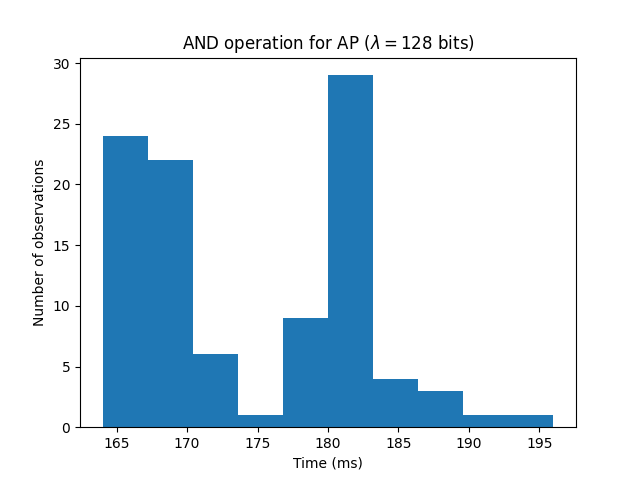
\includegraphics[width=0.8\linewidth]{data/figures/AP_STD128_AND_operation.png}
    \caption{Time distribution when doing Test S4 (AND operation) in Chapter \ref{sec:efficiency_tests} for 128 bits secure AP 100 times.}
    \label{fig:distr_ap128_and}
\end{figure}

\begin{figure}[ht]
    \centering
    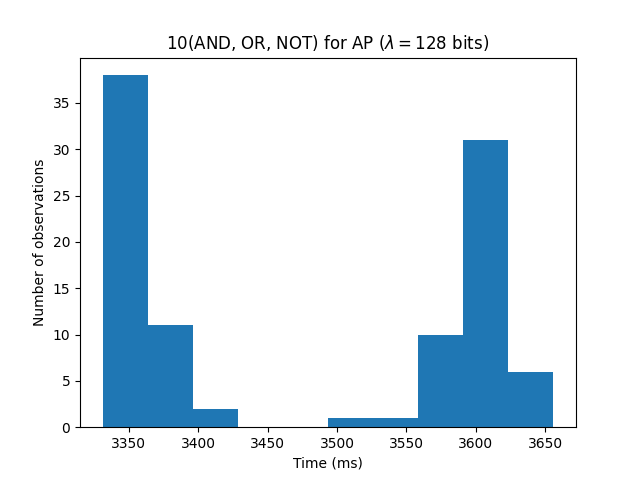
\includegraphics[width=0.8\linewidth]{data/figures/AP_STD128_10AND_OR_NOT.png}
    \caption{Time distribution when doing Test B2 in Chapter \ref{sec:efficiency_tests} consisting of 10 AND, OR, and NOT operations for 128 bits secure AP 100 times.}
    \label{fig:distr_ap128_10}
\end{figure}

%%%%%%%% GINX 128 %%%%%%%%
\begin{figure}[ht]
    \centering
    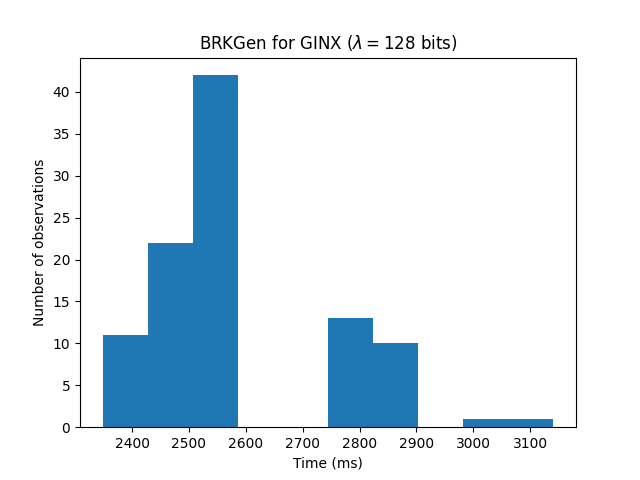
\includegraphics[width=0.8\linewidth]{data/figures/GINX_STD128_BRKGen.png}
    \caption{Time distribution when doing Test S1 (key generation) in Chapter \ref{sec:efficiency_tests} for 128 bits secure GINX 100 times.}
    \label{fig:distr_ginx128_keygen}
\end{figure}

\begin{figure}[ht]
    \centering
    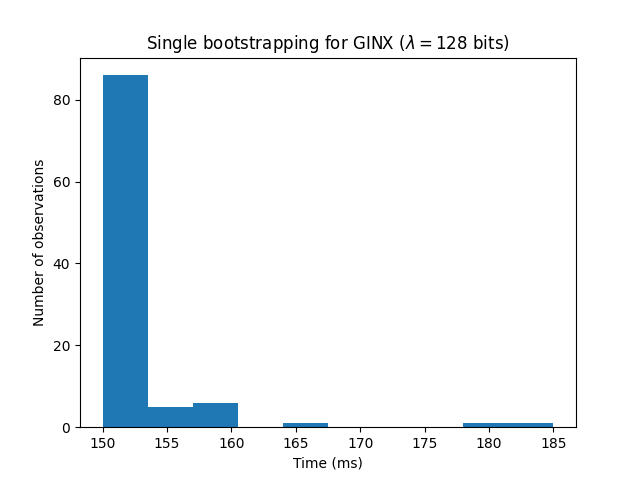
\includegraphics[width=0.8\linewidth]{data/figures/GINX_STD128_Single_bootstrapping.png}
    \caption{Time distribution when doing Test S2 (single bootstrapping operation) in Chapter \ref{sec:efficiency_tests} for 128 bits secure GINX 100 times.}
    \label{fig:distr_ginx128_bs}
\end{figure}

\begin{figure}[ht]
    \centering
    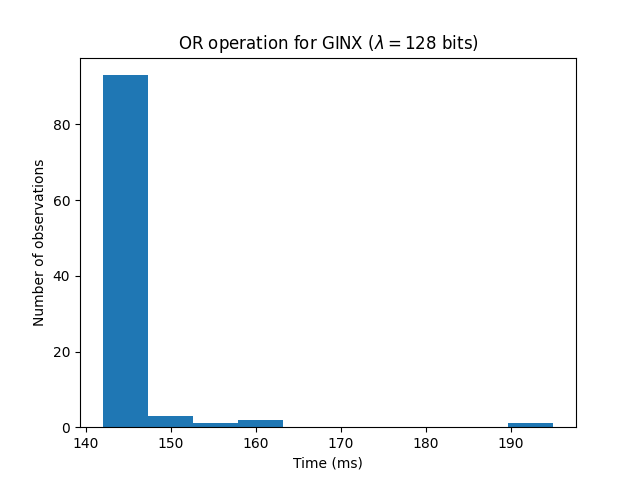
\includegraphics[width=0.8\linewidth]{data/figures/GINX_STD128_OR_operation.png}
    \caption{Time distribution when doing Test S3 (OR operation) in Chapter \ref{sec:efficiency_tests} for 128 bits secure GINX 100 times.}
    \label{fig:distr_ginx128_or}
\end{figure}

\begin{figure}[ht]
    \centering
    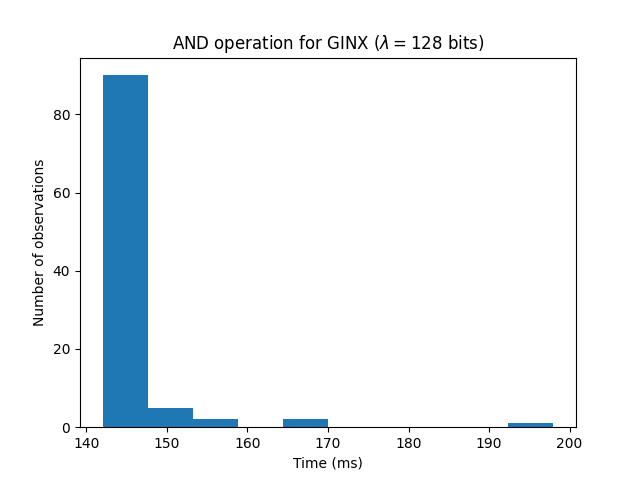
\includegraphics[width=0.8\linewidth]{data/figures/GINX_STD128_AND_operation.png}
    \caption{Time distribution when doing Test S4 (AND operation) in Chapter \ref{sec:efficiency_tests} for 128 bits secure GINX 100 times.}
    \label{fig:distr_ginx128_and}
\end{figure}

\begin{figure}[ht]
    \centering
    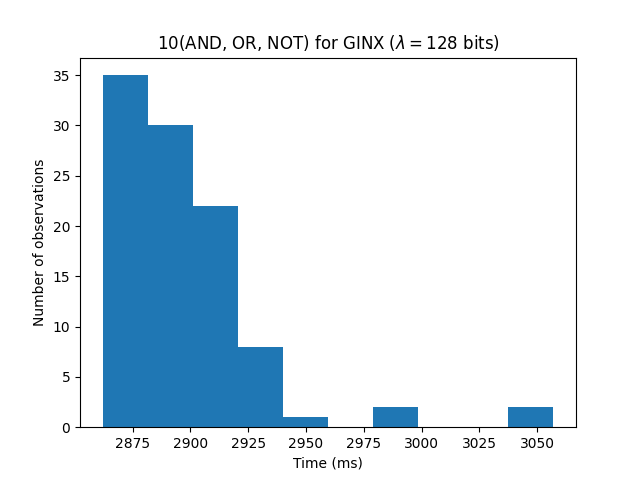
\includegraphics[width=0.8\linewidth]{data/figures/GINX_STD128_10AND_OR_NOT.png}
    \caption{Time distribution when doing Test B2 in Chapter \ref{sec:efficiency_tests} consisting of 10 AND, OR, and NOT operations for 128 bits secure GINX 100 times.}
    \label{fig:distr_ginx128_10}
\end{figure}

%%%%%%%% LMKCDEY 128 %%%%%%%%
\begin{figure}[ht]
    \centering
    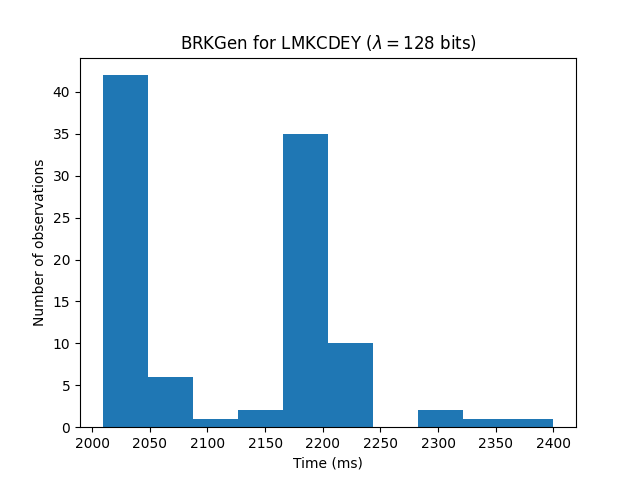
\includegraphics[width=0.8\linewidth]{data/figures/LMKCDEY_STD128LMKCDEY_BRKGen.png}
    \caption{Time distribution when doing Test S1 (key generation) in Chapter \ref{sec:efficiency_tests} for 128 bits secure LMKCDEY 100 times.}
    \label{fig:distr_lmkcdey128_keygen}
\end{figure}

\begin{figure}[ht]
    \centering
    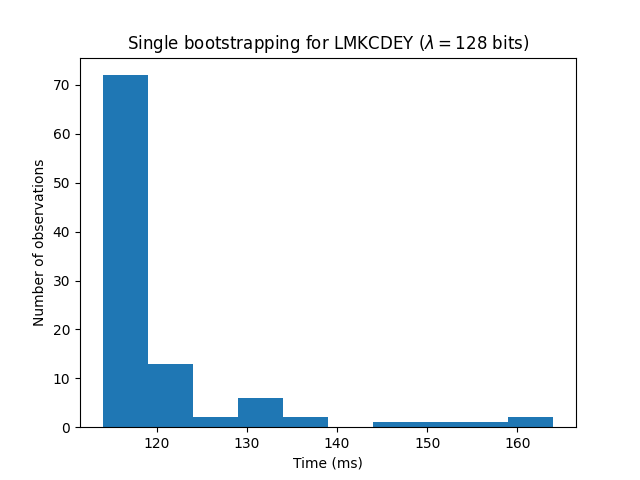
\includegraphics[width=0.8\linewidth]{data/figures/LMKCDEY_STD128LMKCDEY_Single_bootstrapping.png}
    \caption{Time distribution when doing Test S2 (single bootstrapping operation) in Chapter \ref{sec:efficiency_tests} for 128 bits secure LMKCDEY 100 times.}
    \label{fig:distr_lmkcdey128_bs}
\end{figure}

\begin{figure}[ht]
    \centering
    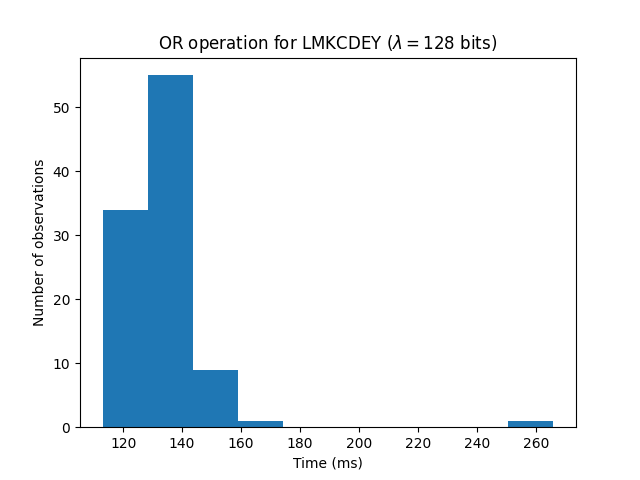
\includegraphics[width=0.8\linewidth]{data/figures/LMKCDEY_STD128LMKCDEY_OR_operation.png}
    \caption{Time distribution when doing Test S3 (OR operation) in Chapter \ref{sec:efficiency_tests} for 128 bits secure LMKCDEY 100 times.}
    \label{fig:distr_lmkcdey128_or}
\end{figure}

\begin{figure}[ht]
    \centering
    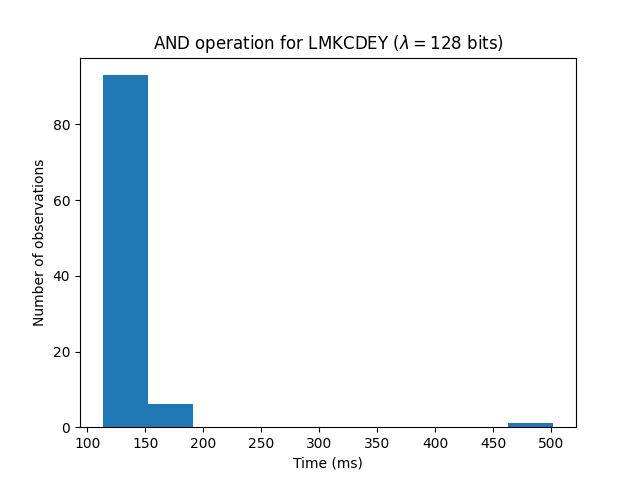
\includegraphics[width=0.8\linewidth]{data/figures/LMKCDEY_STD128LMKCDEY_AND_operation.png}
    \caption{Time distribution when doing Test S4 (AND operation) in Chapter \ref{sec:efficiency_tests} for 128 bits secure LMKCDEY 100 times.}
    \label{fig:distr_lmkcdey128_and}
\end{figure}

\begin{figure}[ht]
    \centering
    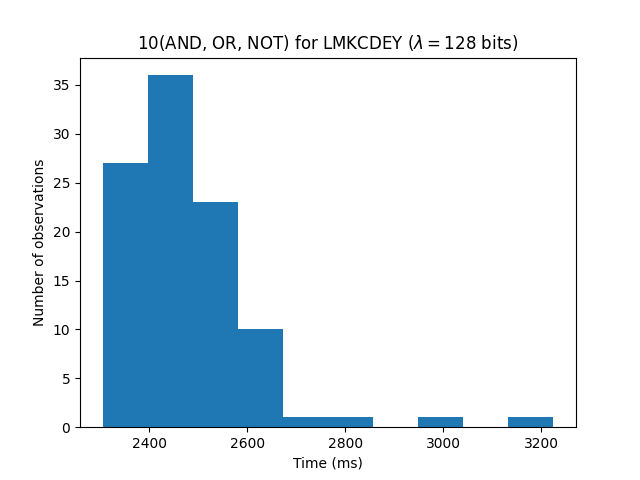
\includegraphics[width=0.8\linewidth]{data/figures/LMKCDEY_STD128LMKCDEY_10AND_OR_NOT.png}
    \caption{Time distribution when doing Test B2 in Chapter \ref{sec:efficiency_tests} consisting of 10 AND, OR, and NOT operations for 128 bits secure LMKCDEY 100 times.}
    \label{fig:distr_lmkcdey128_10}
\end{figure}

%%%%%%%% XZDDF 128 %%%%%%%%
\begin{figure}[ht]
    \centering
    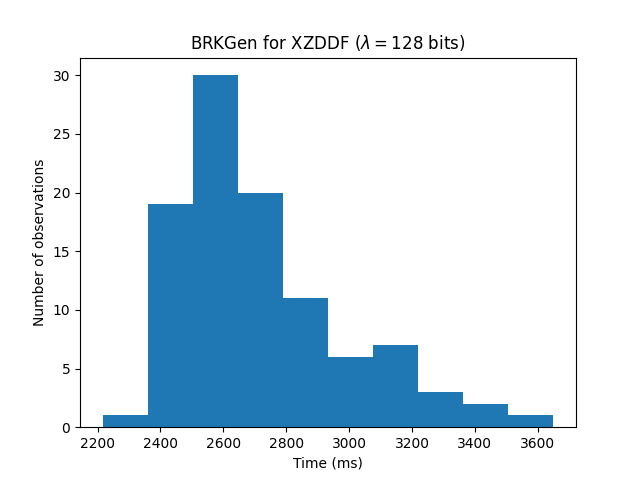
\includegraphics[width=0.8\linewidth]{data/figures/XZDDF_STD128_BRKGen.png}
    \caption{Time distribution when doing Test S1 (key generation) in Chapter \ref{sec:efficiency_tests} for 128 bits secure XZDDF 100 times.}
    \label{fig:distr_xzddf128_keygen}
\end{figure}

\begin{figure}[ht]
    \centering
    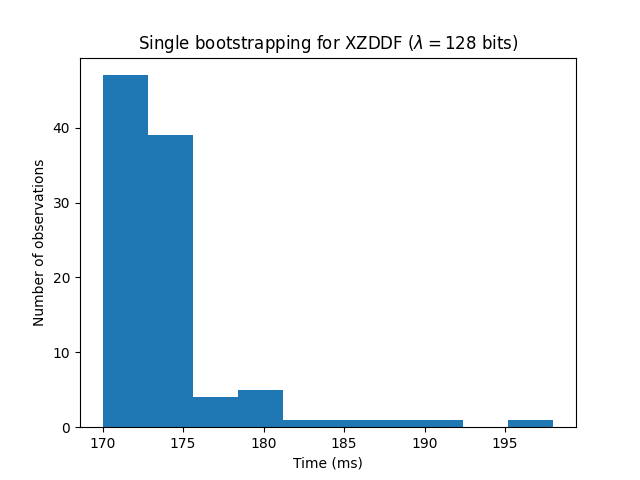
\includegraphics[width=0.8\linewidth]{data/figures/XZDDF_STD128_Single_bootstrapping.png}
    \caption{Time distribution when doing Test S2 (single bootstrapping operation) in Chapter \ref{sec:efficiency_tests} for 128 bits secure XZDDF 100 times.}
    \label{fig:distr_xzddf128_bs}
\end{figure}

\begin{figure}[ht]
    \centering
    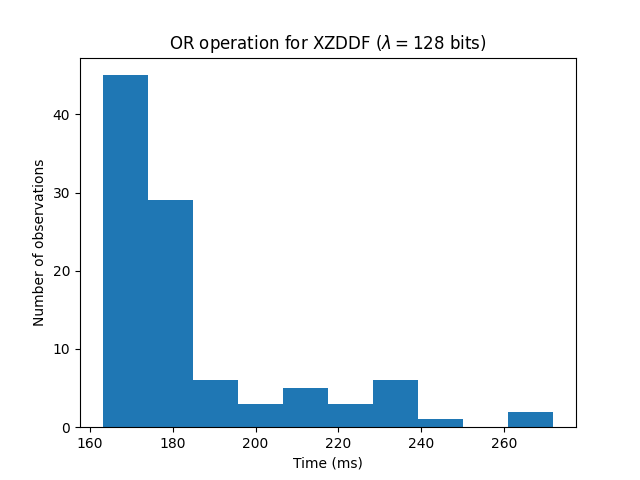
\includegraphics[width=0.8\linewidth]{data/figures/XZDDF_STD128_OR_operation.png}
    \caption{Time distribution when doing Test S3 (OR operation) in Chapter \ref{sec:efficiency_tests} for 128 bits secure XZDDF 100 times.}
    \label{fig:distr_xzddf128_or}
\end{figure}

\begin{figure}[ht]
    \centering
    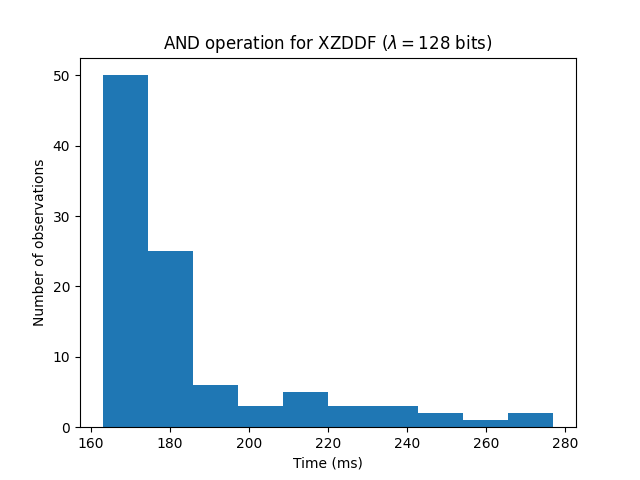
\includegraphics[width=0.8\linewidth]{data/figures/XZDDF_STD128_AND_operation.png}
    \caption{Time distribution when doing Test S4 (AND operation) in Chapter \ref{sec:efficiency_tests} for 128 bits secure XZDDF 100 times.}
    \label{fig:distr_xzddf128_and}
\end{figure}

\begin{figure}[ht]
    \centering
    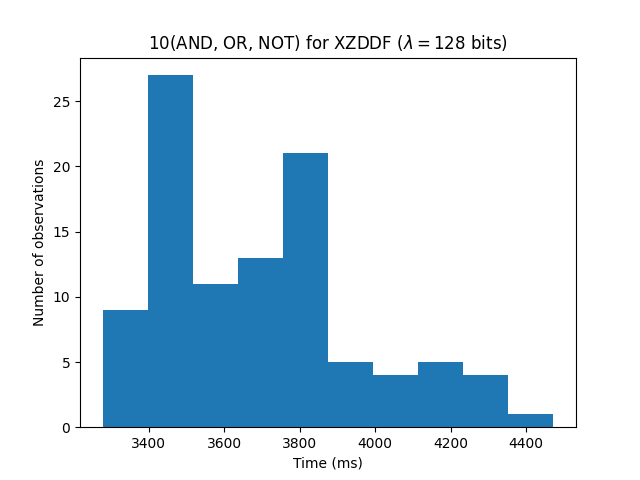
\includegraphics[width=0.8\linewidth]{data/figures/XZDDF_STD128_10AND_OR_NOT.png}
    \caption{Time distribution when doing Test B2 in Chapter \ref{sec:efficiency_tests} consisting of 10 AND, OR, and NOT operations for 128 bits secure XZDDF 100 times.}
    \label{fig:distr_xzddf128_10}
\end{figure}







%%%%%%%% AP 192 %%%%%%%%
\begin{figure}[ht]
    \centering
    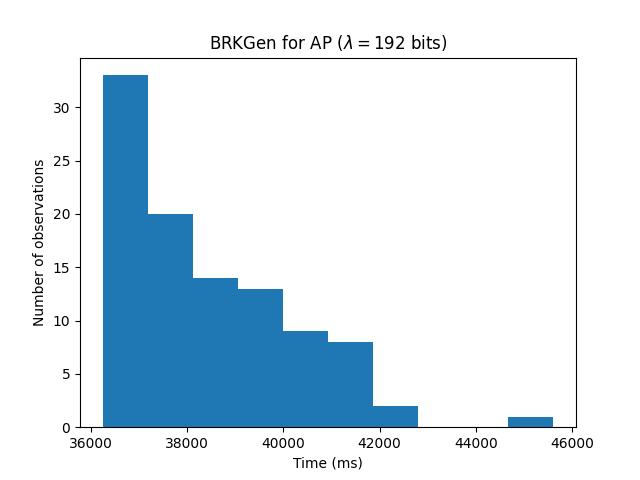
\includegraphics[width=0.8\linewidth]{data/figures/AP_STD192_BRKGen.png}
    \caption{Time distribution when doing Test S1 (key generation) in Chapter \ref{sec:efficiency_tests} for 192 bits secure AP 100 times.}
    \label{fig:distr_ap192_keygen}
\end{figure}

\begin{figure}[ht]
    \centering
    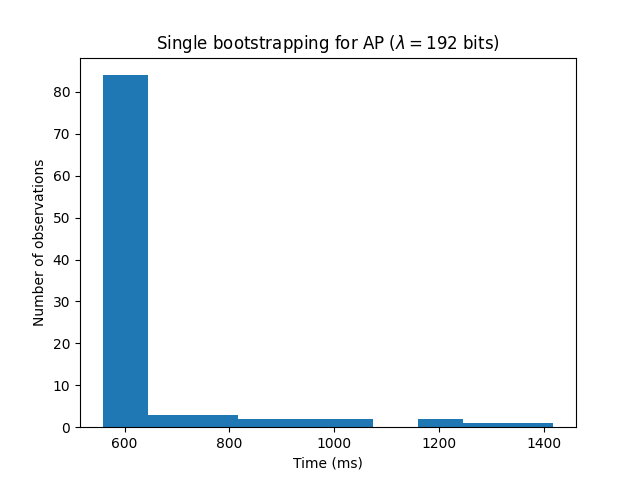
\includegraphics[width=0.8\linewidth]{data/figures/AP_STD192_Single_bootstrapping.png}
    \caption{Time distribution when doing Test S2 (single bootstrapping operation) in Chapter \ref{sec:efficiency_tests} for 192 bits secure AP 100 times.}
    \label{fig:distr_AP192_bs}
\end{figure}

\begin{figure}[ht]
    \centering
    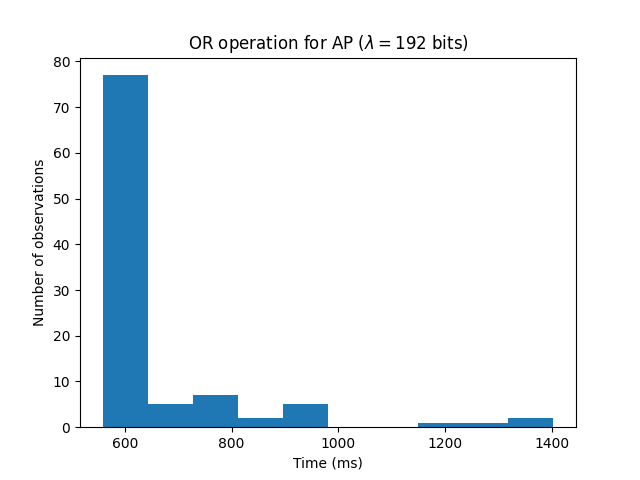
\includegraphics[width=0.8\linewidth]{data/figures/AP_STD192_OR_operation.png}
    \caption{Time distribution when doing Test S3 (OR operation) in Chapter \ref{sec:efficiency_tests} for 192 bits secure AP 100 times.}
    \label{fig:distr_ap192_or}
\end{figure}

\begin{figure}[ht]
    \centering
    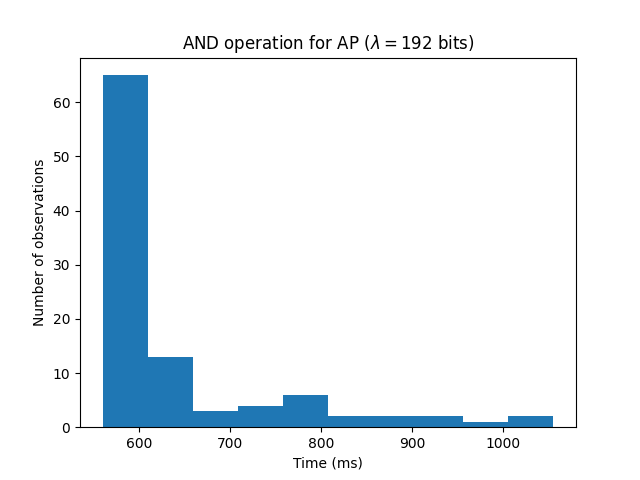
\includegraphics[width=0.8\linewidth]{data/figures/AP_STD192_AND_operation.png}
    \caption{Time distribution when doing Test S4 (AND operation) in Chapter \ref{sec:efficiency_tests} for 192 bits secure AP 100 times.}
    \label{fig:distr_ap192_and}
\end{figure}

\begin{figure}[ht]
    \centering
    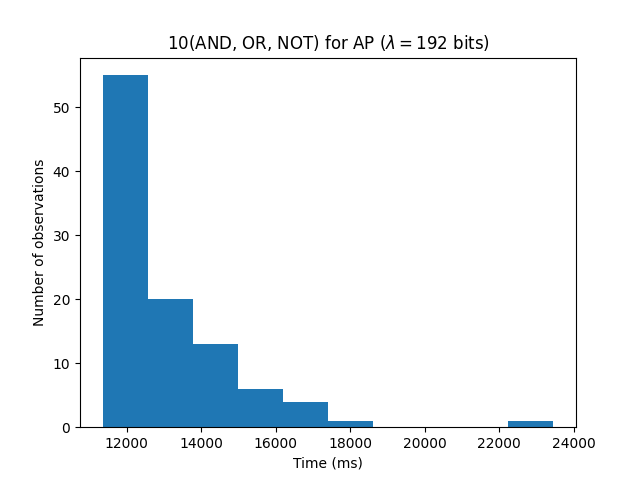
\includegraphics[width=0.8\linewidth]{data/figures/AP_STD192_10AND_OR_NOT.png}
    \caption{Time distribution when doing Test B2 in Chapter \ref{sec:efficiency_tests} consisting of 10 AND, OR, and NOT operations for 192 bits secure AP 100 times.}
    \label{fig:distr_ap192_10}
\end{figure}

%%%%%%%% GINX 192 %%%%%%%%
\begin{figure}[ht]
    \centering
    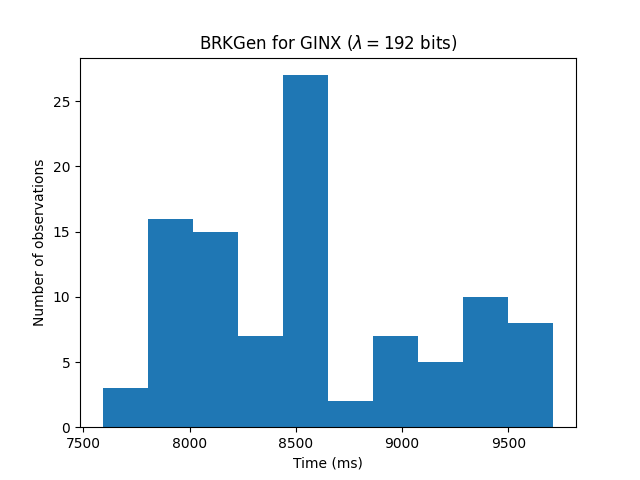
\includegraphics[width=0.8\linewidth]{data/figures/GINX_STD192_BRKGen.png}
    \caption{Time distribution when doing Test S1 (key generation) in Chapter \ref{sec:efficiency_tests} for 192 bits secure GINX 100 times.}
    \label{fig:distr_ginx192_keygen}
\end{figure}

\begin{figure}[ht]
    \centering
    \includegraphics[width=0.8\linewidth]{data/figures/GINX_STD192_Single_bootstrapping.png}
    \caption{Time distribution when doing Test S2 (single bootstrapping operation) in Chapter \ref{sec:efficiency_tests} for 192 bits secure GINX 100 times.}
    \label{fig:distr_ginx192_bs}
\end{figure}

\begin{figure}[ht]
    \centering
    \includegraphics[width=0.8\linewidth]{data/figures/GINX_STD192_OR_operation.png}
    \caption{Time distribution when doing Test S3 (OR operation) in Chapter \ref{sec:efficiency_tests} for 192 bits secure GINX 100 times.}
    \label{fig:distr_ginx192_or}
\end{figure}

\begin{figure}[ht]
    \centering
    \includegraphics[width=0.8\linewidth]{data/figures/GINX_STD192_AND_operation.png}
    \caption{Time distribution when doing Test S4 (AND operation) in Chapter \ref{sec:efficiency_tests} for 192 bits secure GINX 100 times.}
    \label{fig:distr_ginx192_and}
\end{figure}

\begin{figure}[ht]
    \centering
    \includegraphics[width=0.8\linewidth]{data/figures/GINX_STD192_10AND_OR_NOT.png}
    \caption{Time distribution when doing Test B2 in Chapter \ref{sec:efficiency_tests} consisting of 10 AND, OR, and NOT operations for 192 bits secure GINX 100 times.}
    \label{fig:distr_ginx192_10}
\end{figure}

%%%%%%%% LMKCDEY 192 %%%%%%%%
\begin{figure}[ht]
    \centering
    \includegraphics[width=0.8\linewidth]{data/figures/LMKCDEY_STD192_BRKGen.png}
    \caption{Time distribution when doing Test S1 (key generation) in Chapter \ref{sec:efficiency_tests} for 192 bits secure LMKCDEY 100 times.}
    \label{fig:distr_lmkcdey192_keygen}
\end{figure}

\begin{figure}[ht]
    \centering
    \includegraphics[width=0.8\linewidth]{data/figures/LMKCDEY_STD192_Single_bootstrapping.png}
    \caption{Time distribution when doing Test S2 (single bootstrapping operation) in Chapter \ref{sec:efficiency_tests} for 192 bits secure LMKCDEY 100 times.}
    \label{fig:distr_lmkcdey192_bs}
\end{figure}

\begin{figure}[ht]
    \centering
    \includegraphics[width=0.8\linewidth]{data/figures/LMKCDEY_STD192_OR_operation.png}
    \caption{Time distribution when doing Test S3 (OR operation) in Chapter \ref{sec:efficiency_tests} for 192 bits secure LMKCDEY 100 times.}
    \label{fig:distr_lmkcdey192_or}
\end{figure}

\begin{figure}[ht]
    \centering
    \includegraphics[width=0.8\linewidth]{data/figures/LMKCDEY_STD192_AND_operation.png}
    \caption{Time distribution when doing Test S4 (AND operation) in Chapter \ref{sec:efficiency_tests} for 192 bits secure LMKCDEY 100 times.}
    \label{fig:distr_lmkcdey192_and}
\end{figure}

\begin{figure}[ht]
    \centering
    \includegraphics[width=0.8\linewidth]{data/figures/LMKCDEY_STD192_10AND_OR_NOT.png}
    \caption{Time distribution when doing Test B2 in Chapter \ref{sec:efficiency_tests} consisting of 10 AND, OR, and NOT operations for 192 bits secure LMKCDEY 100 times.}
    \label{fig:distr_lmkcdey192_10}
\end{figure}

%%%%%%%% XZDDF 192 %%%%%%%%
\begin{figure}[ht]
    \centering
    \includegraphics[width=0.8\linewidth]{data/figures/XZDDF_STD192_BRKGen.png}
    \caption{Time distribution when doing Test S1 (key generation) in Chapter \ref{sec:efficiency_tests} for 192 bits secure XZDDF 100 times.}
    \label{fig:distr_xzddf192_keygen}
\end{figure}

\begin{figure}[ht]
    \centering
    \includegraphics[width=0.8\linewidth]{data/figures/XZDDF_STD192_Single_bootstrapping.png}
    \caption{Time distribution when doing Test S2 (single bootstrapping operation) in Chapter \ref{sec:efficiency_tests} for 192 bits secure XZDDF 100 times.}
    \label{fig:distr_xzddf192_bs}
\end{figure}

\begin{figure}[ht]
    \centering
    \includegraphics[width=0.8\linewidth]{data/figures/XZDDF_STD192_OR_operation.png}
    \caption{Time distribution when doing Test S3 (OR operation) in Chapter \ref{sec:efficiency_tests} for 192 bits secure XZDDF 100 times.}
    \label{fig:distr_xzddf192_or}
\end{figure}

\begin{figure}[ht]
    \centering
    \includegraphics[width=0.8\linewidth]{data/figures/XZDDF_STD192_AND_operation.png}
    \caption{Time distribution when doing Test S4 (AND operation) in Chapter \ref{sec:efficiency_tests} for 192 bits secure XZDDF 100 times.}
    \label{fig:distr_xzddf192_and}
\end{figure}

\begin{figure}[ht]
    \centering
    \includegraphics[width=0.8\linewidth]{data/figures/XZDDF_STD192_10AND_OR_NOT.png}
    \caption{Time distribution when doing Test B2 in Chapter \ref{sec:efficiency_tests} consisting of 10 AND, OR, and NOT operations for 192 bits secure XZDDF 100 times.}
    \label{fig:distr_xzddf192_10}
\end{figure}





%%%%%%%%%%%%%%%%%%%%%%%%%%%%%
%%%%%%%% Batch tests %%%%%%%%
%%%%%%%%%%%%%%%%%%%%%%%%%%%%%

\begin{figure}[ht]
    \centering
    \includegraphics[width=0.8\linewidth]{data/figures/AP_STD128_batch.png}
    \caption{Log-log plot of the average execution times in the batch tests B1--B4 in Chapter \ref{sec:efficiency_tests} consisting of $x$ AND, OR, and NOT operations, for 128 bits secure AP.}
    \label{fig:batch_ap128}
\end{figure}

\begin{figure}[ht]
    \centering
    \includegraphics[width=0.8\linewidth]{data/figures/GINX_STD128_batch.png}
    \caption{Log-log plot of the average execution times in the batch tests B1--B4 in Chapter \ref{sec:efficiency_tests} consisting of $x$ AND, OR, and NOT operations, for 128 bits secure GINX.}
    \label{fig:batch_ginx128}
\end{figure}

\begin{figure}[ht]
    \centering
    \includegraphics[width=0.8\linewidth]{data/figures/LMKCDEY_STD128LMKCDEY_batch.png}
    \caption{Log-log plot of the average execution times in the batch tests B1--B4 in Chapter \ref{sec:efficiency_tests} consisting of $x$ AND, OR, and NOT operations, for 128 bits secure LMKCDEY.}
    \label{fig:batch_lmkcdey128}
\end{figure}

\begin{figure}[ht]
    \centering
    \includegraphics[width=0.8\linewidth]{data/figures/XZDDF_STD128_batch.png}
    \caption{Log-log plot of the average execution times in the batch tests B1--B4 in Chapter \ref{sec:efficiency_tests} consisting of $x$ AND, OR, and NOT operations, for 128 bits secure XZDDF.}
    \label{fig:batch_xzddf128}
\end{figure}


\begin{figure}[ht]
    \centering
    \includegraphics[width=0.8\linewidth]{data/figures/AP_STD192_batch.png}
    \caption{Log-log plot of the average execution times in the batch tests B1--B4 in Chapter \ref{sec:efficiency_tests} consisting of $x$ AND, OR, and NOT operations, for 192 bits secure AP.}
    \label{fig:batch_ap192}
\end{figure}

\begin{figure}[ht]
    \centering
    \includegraphics[width=0.8\linewidth]{data/figures/GINX_STD192_batch.png}
    \caption{Log-log plot of the average execution times in the batch tests B1--B4 in Chapter \ref{sec:efficiency_tests} consisting of $x$ AND, OR, and NOT operations, for 192 bits secure GINX.}
    \label{fig:batch_ginx192}
\end{figure}

\begin{figure}[ht]
    \centering
    \includegraphics[width=0.8\linewidth]{data/figures/LMKCDEY_STD192_batch.png}
    \caption{Log-log plot of the average execution times in the batch tests B1--B4 in Chapter \ref{sec:efficiency_tests} consisting of $x$ AND, OR, and NOT operations, for 192 bits secure LMKCDEY.}
    \label{fig:batch_lmkcdey192}
\end{figure}

\begin{figure}[ht]
    \centering
    \includegraphics[width=0.8\linewidth]{data/figures/XZDDF_STD192_batch.png}
    \caption{Log-log plot of the average execution times in the batch tests B1--B4 in Chapter \ref{sec:efficiency_tests} consisting of $x$ AND, OR, and NOT operations, for 192 bits secure XZDDF.}
    \label{fig:batch_xzddf192}
\end{figure}

\fi